\documentclass[../ImageClassifier.tex]{subfiles}

\begin{document}
    Fine tuning is used in this project to get the last small improvements of a network.
    For that, all layers of the network are set to trainable and the learning is set to very low (1e-5).
    The low learning rate prevents the excessive change of weights in the network and is good to get the final optimization for the network, because with higher learning rates the weights oscillates to much.
    This implementation is only experimental and the fine tuned model will be only saved, if the validation loss is better than the saved model.
    On my tested keywords there was no benefit with fine tuning for example as shown in figure \ref{fig:training result calculator,pen,triangle ruler}, but it cannot cause any damage and if it worser than the pre-saved transfer learning model, it has no effect on the model.
    \begin{figure}[ht!]
        \centering
        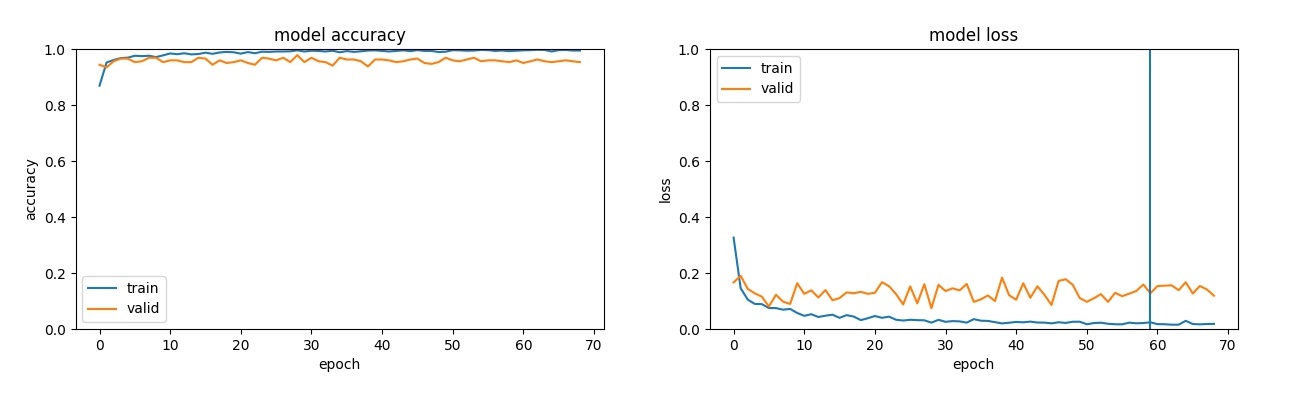
\includegraphics[width=1\linewidth]{./attachments/fine tuning/calculator,pen,triangle ruler.jpg}
        \caption{Training result of keywords calculator, pen and triangle ruler}
        \label{fig:training result calculator,pen,triangle ruler}
    \end{figure}
\end{document}